\chapter{Components}
\label{chap:components}
% we have described many technologies in previous cgapters
% for our architecture we have chosen the following technologies
% they will be discussed in greater details

% storage/persistent streeming/real time processing scala(or additional technologies/surrounding)

\authorsection{Storage systems}{SP}

\subsection{HDFS}

\subsection{Redys}

\authorsection{Real time processing systems}{SP}

\subsection{Storm}
Batch processing is not applicable for real time computing.
Hadoop, the best known tool for batch processing, is helpless when it is needed to handle streaming data and obtain immediate result.
The main advantage of real time processing, the guaranteed time delay between a request and a result can be broken simply because the waiting time for the next batch is too long.
Therefore new systems, designed for real-time processing, have appeared.
One of such systems is an open source project named \textit{Storm}.

Storm is a \textit{complex event-processing} (CEP) system.
Complex event processing means gathering data from different sources, combining it and making conclusions from it.
For example, such system keeps track of significant changes in traffic reports or stock market feeds and immediately responds to them. 

Storm is implemented in a dialect of the Lisp language named Clojure.
Clojure is a functional language like Lisp, but it also supports multithreaded programming.
Clojure runs on the Java Virtual Machine, however applications within Storm can be written in Java, Scala, JRuby, Perl and PHP.
Moreover, one can use a Structured Query Language adapter for streaming data directly into Storm topoloy.

\mnote{Storm architecture}
The Storm cluster has a master node called \textit{Nimbus} and \textit{worker} nodes.
Nimbus assignes tasks for workers and monitors failures.
There is a deamon called \textit{Supervisor} on every worker node.
The supervisor is responsible for starting and stopping worker processes assigned by Nimbus.
ZooKeeper coordinates the interaction between Nimbus and Supervisors.
It stores the state of all the nodes, making the system stable to failures.
If any of the nodes is killed, ZooKeeper immediately restarts it, enhancing Storm cluster stability.
ZooKeeper is described in more details later in this chapter.

The basic concept of Storm is a \textit{topology}.
It is a graph of computation, that shows how data should be processed and passed between the nodes.
One can implement a topology in any programming language, because topology definition is a Thrift structure.
Thrift is a framework that allows to develop cross-language services.	

The data stream consists of an unbounded set of \textit{tuples}.
A tuple can contain both standard data types (integer, float, byte array) as well as user-defined types.
Every stream has its own ID.
The sources of streams called \textit{spouts}. 

The next important Storm primitive is \textit{bolt}.
Figure~\ref{fig:storm_architecture} shows the interaction between spouts and bolts.
The stream of tuples originates from a spout and goes through a sequence of bolts.
Every bolt performs a transformation on incoming data stream, like aggregating, filtering, or interaction with external parts such as databases.
A bolt can receive information from several spouts and stream it to multiple bolts.

\begin{figure}
  \centering
  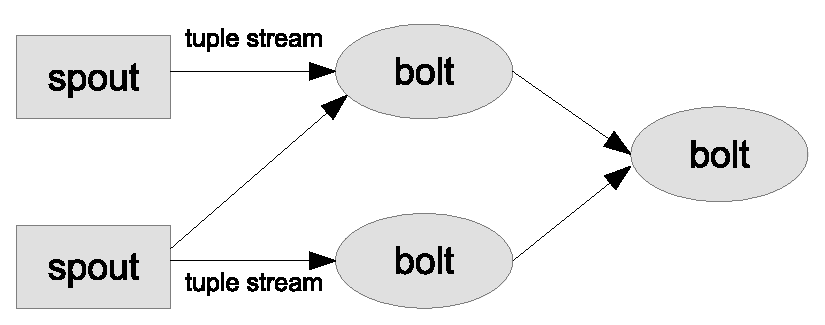
\includegraphics [width=0.5\textwidth]{images/storm_architecture}
  \caption{Storm architecture}
  \label{fig:storm_architecture}
\end{figure}

For example, MapReduce word counting example can be easily implemented with Storm.
Such system counts how many times each word occures in a given input data.
In the case of Storm one needs 
(1) a spout to generate text data, 
(2) one bolt to implement the Map function for word tokenisation and 
(3) one bolt to implement the Reduce function for aggregation the amounts of words occurences. 

Storm allows to group the stream of tuples in different ways.
For instance, shuffle grouping randomly distributes tuples to bolts such as each bolt receives approximately the same number of tuples.
Field grouping partitions tuples according to contained fields.
Also other grouping methods exist, including the custom grouping.

The Listing~\ref{lis:simple_storm_topology} represents a simple topology.

\begin{lstlisting}[caption=Simple Storm topology, label=lis:simple_storm_topology]
java TopologyBuilder builder = new TopologyBuilder();
builder.setSpout("myspout", new TestSpout(), 10);
builder.setBolt("mybolt1", new TestBolt(), 3) .shuffleGrouping("myspout");
builder.setBolt("mybolt2", new TestBolt(), 2) .shuffleGrouping("mybolt1");
\end{lstlisting}

Here topology consists of one spout and two bolts.
The stream of tuples originates from \textit{myspout}, then it is passed to \textit{mybolt1} and finally to \textit{mybolt2}.
In both cases tuples are grupped using the schuffle grouping method.
The integer numbers in \textit{setSpout} and \textit{setBolt} define the amount of parallelism for the node.

The implementation charasteristics of Storm lead to high performance and guaranteed fault tolerance.
It uses ZeroMQ for passing messages between the tasks.
Messages are automatically serialized and deserialized to Storm primitive types.
The usage of this message queue helps to avoid intermediate queueing, thus improving performance.
Furthermore, Storm guarantees the processing of every tuple.
In the case of a fault during message processing, a tuple is replayed from the spout.
There is also a fault detection mechanism on task level, when the failed task is quickly reassigned to restart the processing.
Storm has supervisors to manage the processes, that leads to efficient usage of resources.

Storm cooperates with message queue systems in such a way that every message is fully processed.
It builds a tuple tree, that reflects the motion af all the tuples.
Only when every message in the tuple tree is processed, a tuple is considered to be fully processed.

To give an example, let us take a message queue that supplies a spout with messages.
When the spout takes a message from the queue, the message state changes to 'pending'.
In this state it cannot be sent to other consumers.
Moreover, all the messages in pending state are returned to message queue if their consumer disconnects.
Storm assignes a unique id to the message, if it is not given by the message queue.
Using this id Storm can keep track of this message during processing.
The system receives this message when the \textit{nextTuple} method of the spout is called.
The spout emits the message along with its id to the consuming bolts.
When a tuple is fully processed, the \textit{ack} method of the original spout is called. 
In the case of time-out Storm calls the \textit{fail} method of the same spout.
Only when \textit{ack} or \textit{fail} method is called, the spout sends an ack or fail message to the message queue.
The message queue cancels the pending state of the message, taking it off the queue in the case of success and putting it back otherwise.

Storm can process not only the tuple trees, but also directed acyclic graphs.
It happens when an output tuple is anchored to several input tuples.
\textit{To anchor} means to specify a link in the tuple tree.
Multi-anchored tuples often appear during streaming aggregation or joining.
 
As it was mentioned, Storm tracks every tuple using its unique id.
Additionally, as each tuple exists within a tree, it knows all the tuples ids of this tree.
For example, if a bolt emits a new tuple, this tuple carries the ids of spout tuples received by this bolt along with its own id.
Such storage mechanism is used	because when the tuple is acked or failed, it should inform Storm about its dependencies to restore the state of the tuple tree.  

The acker task is responsible for acking the tuple.
First, Strom stores the mapping between an acker task and a spout tuple id.
As every tuple keeps ids of spout tuples in the tree it exists within, it knows the acker tasks it should communicate with.
A tuple informs an acker task when the tree is fully processed and the tuple is acked.
Second, the acker task should send a complition message to the spout task that emitted this tuple.
For this purpose, on creation of a new tuple a spout task notifies the appropriate acker task that its task id is linked to that spout tuple.

For acker task tracking the huge tuple trees explicitly is not efficient.
Thus Storm uses a special tracking strategy.
An acker task stores a map: on the one side it has a spout tuple id and on the other side a pair of values.
One of the values is a task id the spout tuple originates from, and the other is an 'ack val', the 64 bit number.
The 'ack val' represents the state of the tuple tree without storing it in memory.
This number is a result of XOR operation on all created and acked tuple ids of the tree.
Therefore, when the 'ack val' is equal to zero, it means that the tree is completed.  

\subsection{Spark}


\authorsection{Surrounding technologies}{SP}

\subsection{Avro + parquet}

\subsection{Scala}

\subsection{Kafka}

\subsection{ZooKeeper}
Large distributed systems require a coordinator for system configuration management.
As it was mentioned in Chapter 4, Google uses a Chubby service for this purpose.
The main Chubby disadvantage is that for lock and unlock operations it is necessary to open and close the object consequently.
This feature influences the performance, increasing the time needed for making a lock.
Therefore Yahoo developes its own service named ZooKeeper that manages systems configuration and allows to efficiently lock the shared resources.

ZooKeeper namespace looks similar to a standard file system.
It consists of interconnected nodes, each of them identified by a path.
The path contains elements separated by a slash ('/').
Like in a file system, every node except the root has a parent node.
The parent node's path is a prefix for the current node path.
The ZooKeeper namespace differs from a standard file system in that its node can be a file and a directory simultaneously.

There are two types of nodes: persistent and ephemeral.
ZooKeeper stores persistent nodes on the disk, while ephemeral nodes belong to a particular session and exist only during this session.
Ephemeral nodes cannot have children nodes, they can only store data.
ZooKeeper client establishes a session with a ZooKeeper server, passing heartbeat messages.
When a client stopes to receive heartbeat messages, it reconnects to a defferent server, reestablishing the session.
If the session is canceled, all its ephemeral nodes are automatically removed.
ZooKeeper tree is presented in Figure~\ref{fig:zookeeper_tree} where the dark nodes are ephemeral.

\begin{figure}
  \centering
  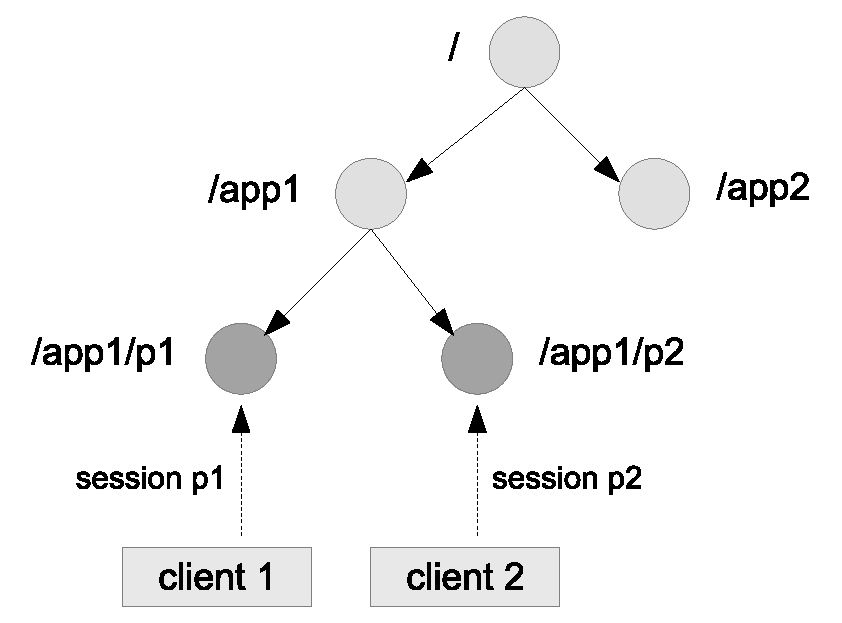
\includegraphics [width=0.5\textwidth]{images/zookeeper_tree}
  \caption{ZooKeeper tree sructure}
  \label{fig:zookeeper_tree}
\end{figure}

ZooKeeper is designed for small data warehousing, such as configuration, status and location information.
One node is usually not bigger than one kilobyte.
Therefore it stores data tree image in memory, keeping in a persistent store only transaction logs and snapshots.
In-memory storage limits the size of the database of ZooKeeper.
However, it gives advantages of low latency and high performance. 

The key feature of ZooKeeper is that it uses First In, First Out (FIFO) method for processing the messages.
It means that all commands are performed in the order they are received.
Thus, ZooKeeper maintains the total ordering.
The order is specified by a unique ZooKeeper Transaction id, that is assigned to each update.
 
ZooKeeper supports idempotent operations.
If a node should be updated, the system makes a note about the update and keeps an old and a new version of this node.
This allows client to receive the same message several times, being aware of when it can be applied.
Therefore all the write operations are performed sequentially in one thread and only on the master node.
On the contrary, read requests do not necessarily need the master node, they can be handled by a node's replica.

The client also supports the total ordering of the messages.
Hence if the client sends a write request and then a read request, the write operation is performed first.
Even if usually read operation does not need a lock, ZooKeeper strictly follows the order.
It allows to implement predictable asynchronous systems that work with ZooKeeper.

A client can watch a node.
If it sets a watch, it gets notified when the node is changed.
When the node sends this notification, it removes the watch.
In the case of connection problems between the client and the ZooKeeper server, the client receives a local notification.

ZooKeeper guarantees reliability using replication.
Its database is replicated to several nodes, one of them is a \textit{Leader} and the others are \textit{Followers}.
\textit{ZooKeeper Atomic Broadcast} (Zab) algorithm is used for managing the communication between the leader and the followers.
It synchronizes the replicas, broadcasts updates and recovers the valid state in the case of nodes crash.

Zab includes four phases: (1) Leader election, (2) Discovery, (3) Synchronization and (4) Broadcast.

1. On the first stage ZooKeeper uses any election algorithm to choose a leader.
After termination every node stores its vote locally in volatile memory.
When a node \textit{n} votes for a node \textit{n'}, \textit{n'} becomes a \textit{prospective leader} for \textit{n}.

2. On the second stage the nodes inform the prospective leader about the most recent transactions they accepted.
Thus the prospective leader knows the latest sequence af accepted transactions and can establish a new epoch.
From thit moment the previous leaders cannot perform any commits.
In the case of connection problems between a follower and a leader, the follower goes back to the stage (1) of this algorithm.

3. The leader is aware of the latests transactions history and during this stage synchronizes this information with its replicas.
This phase is also called voting phase, because it receives the votes from the nodes.
The leader performes a commit only if it receives acknowledgements from two of three followers.
At this moment the leader changes its state from \textit{prospective} to \textit{established}.

4. The nodes persist in this stage until a crash.
Every write request from a ZooKeeper client is broadcasted among the nodes.
New followers can join, receiving the transaction history from the leader.
The leader and its followers use periodic heartbeat messages for early failure detection.
If any of the nodes does nor receive a heartbeat message within a timeout, it shifts its state to \textit{election} and goes back to the first stage.

It can happened that one of the followers still has an outdated information when it receives the read request.
To avoid this problem, it is possible to make a force synchronisation with the master.
It is called the \textit{slow read}.
Evidently, if all the clients use the slow read the system looses the advantage of scaling.
Without force synchronisation ZooKeeper system scales for reads nicely. 
However, in this case the client that reads from a replica can obtain the outdated information.


\authorsection{Alternatives}{NO}
cassandra?